\documentclass[10pt,a4paper]{article}
\usepackage[T1]{fontenc}
\usepackage{lmodern}
\usepackage[margin=25mm]{geometry}
\usepackage{amsmath,amssymb,booktabs,microtype}
\usepackage{tikz}
\usetikzlibrary{arrows.meta}
\usepackage[hidelinks]{hyperref}
\hypersetup{pdftitle={Nonlinear hydropower scheduling with coupled hydraulics and delayed river networks}}
\newcommand{\R}{\mathbb{R}}
\newcommand{\pos}[1]{[#1]_+}
\newcommand{\dd}{\,\mathrm{d}}
\newcommand{\SOS}{\operatorname{SOS2}}
\title{Nonlinear hydropower scheduling with coupled hydraulics\\
and delayed river networks}
\author{}
\date{}
\begin{document}
\maketitle
\vspace{-2em}
\begin{abstract}
Short-term hydropower scheduling couples discrete operation with the movement
of water and the conversion of hydraulic energy. We give a mixed-integer
nonlinear formulation with finite hydraulic domains for reservoirs, shared pressurized
waterways, generating units, discrete gates, instantaneous channels and
delayed river networks. Storage evolves by an implicit midpoint balance.
Pressure losses and efficiency-dependent generation remain nonlinear;
supplied response curves have explicit interpolation semantics.
Deterministic river transport preserves release pulses through confluences,
whereas distributed transport uses conservative interval mixing.
The solution method combines mixed-integer linear proposals, nonlinear
dispatch, exact algebraic interpolation graphs and spatial branch-and-bound.
Independent chronological integration separates physical acceptance from
the objective-gap certificate of the finite optimization model. The
formulation is implemented in Julia using open-source optimization libraries.
\end{abstract}

\section{The scheduling problem}

A generating schedule must account for water volume and hydraulic head.
Discharging a reservoir removes water, changes its level, and changes the
energy obtained from later discharges. Units also have operating ranges:
an idle unit produces nothing, while a running unit cannot usually sustain
arbitrarily small output. Head-dependent generation and these discrete
operating domains have a long history in nonlinear hydropower
scheduling~\cite{catalao}.

We consider a deterministic horizon with given prices, inflows, equipment
curves and operating restrictions. The physical model is deliberately
quasi-steady. Pressure and discharge equilibrate within each control
interval; reservoir storage evolves between intervals. Tunnel inertia,
water hammer, free-surface river momentum equations, pumping, reserve
products and stochastic decisions are outside its scope. River geometry is
represented by supplied response functions, rather than resolved during
scheduling.

The aim is a single explicit physical optimization problem. Linear
approximations may help choose initial discrete decisions, but they do not
define the delivered schedule's hydraulic feasibility. The final equations
retain head-dependent generation, signed pressure losses and contemporaneous
flow-dependent transport. Exactness below means equivalence to these
declared functions and this time discretization, not exact reproduction of
a real watercourse.

\section{Volumes, heads and connections}
\label{sec:water}

Let $0=\tau_0<\cdots<\tau_T$ be time edges in hours,
$\Delta_t=\tau_{t+1}-\tau_t$, and
$m_t=(\tau_t+\tau_{t+1})/2$, for $t=0,\ldots,T-1$.
Operating inputs are piecewise constant, with changes on control edges.
Use the sets $\mathcal R$ of reservoirs, $\mathcal J$ of pressure junctions,
$\mathcal B$ of prescribed-head boundaries, $\mathcal E$ of tunnels,
$\mathcal C$ of instantaneous channels, $\mathcal G$ of units and
$\mathcal D$ of delayed reaches. Units belong to plants $\mathcal G_p$.
Table~\ref{tab:variables} fixes the principal variables and units.

\begin{table}[ht]
\centering
\caption{Physical variables. Storage and river inventory use time vertices;
other indexed quantities use control intervals.}
\label{tab:variables}
\begin{tabular}{lll}
\toprule
Variable & Meaning & Unit\\
\midrule
$V_{it},W_{rt}$ & Reservoir volume, river water in transit & Mm$^3$\\
$H_{nt},h_{pt}$ & Node head, turbine net head & m\\
$Q_{et},X_{ct},q_{gt}$ & Tunnel, channel, unit discharge & m$^3$/s\\
$R_{rt},d_{rt}$ & Reach entry flow, reservoir withdrawal & m$^3$/s\\
$A_{rt}$ & Volume arriving from a delayed reach & Mm$^3$\\
$P_{gt}$ & Electrical power & MW\\
$u_{gt},U_{pt}$ & Unit and plant operating states & $\{0,1\}$\\
$b_{et},a_{rt}$ & Tunnel position, reservoir outlet opening & $[0,1]$\\
\bottomrule
\end{tabular}
\end{table}

Head measures mechanical energy per unit weight. At a reservoir it is the
water-surface elevation; at a flooded pressure junction it includes pressure
head. Raising a parcel by one metre and losing one metre of head to friction
have the same energy scale. Relative velocities and fixed local losses are
absorbed into the supplied equipment relationships.

The unit conversions are
\begin{equation}
\kappa=\frac{3600}{10^6}=0.0036,\qquad
\gamma=\frac{\rho g}{10^6}=0.00981
\quad(\rho=1000\ {\rm kg/m^3},\ g=9.81\ {\rm m/s^2}).
\label{eq:units}
\end{equation}
Thus $\kappa\Delta q$ is a volume in Mm$^3$, and $\gamma qh$ is hydraulic
power in MW.

Define $F_{nt}$ as the net internal rate entering node $n$, before reservoir
natural inflow. With incidence coefficients positive into a node,
\begin{equation}
F_{nt}=\sum_e B^{E}_{ne}Q_{et}
       +\sum_c B^{C}_{nc}X_{ct}
       +\sum_g B^{G}_{ng}q_{gt}
       +\sum_r D_{nr}\frac{A_{rt}}{\kappa\Delta_t}
       -\sum_r S_{nr}d_{rt}.
\label{eq:incidence}
\end{equation}
$D_{nr}=1$ if reach $r$ delivers into node $n$, and $S_{nr}=1$ if
a reservoir outlet at $n$ supplies it. Other entries are zero.
Tunnel and unit incidence uses the actual water destination:
a river outfall withdraws from its source and injects the named reach,
without immediately crediting the hydraulic target.

Reservoirs and pressure junctions obey, respectively,
\begin{align}
V_{i,t+1}-V_{it}&=\kappa\Delta_t(I_{it}+F_{it}),
&V_{i0}&=V_i^{\rm init}, \label{eq:storage}\\
F_{jt}&=0 \quad(j\in\mathcal J),&
\underline V_{it}&\le V_{it}\le\overline V_{it}
\quad(t=0,\ldots,T). \label{eq:junction}
\end{align}
A junction cannot retain water, so its equation is a balance rather than an
evolution law. Boundaries exchange water with the exterior and have fixed
heads. Reservoir hydraulic heads use midpoint storage:
\begin{equation}
H_{it}=Z_i\!\left(\frac{V_{it}+V_{i,t+1}}2\right),\qquad
\underline H_j\le H_{jt}\le\overline H_j,\qquad
H_{bt}=H_b^{\rm given}.
\label{eq:heads}
\end{equation}
$Z_i$ is an increasing supplied level--volume table, or
$Z_i(V)=z_i+s_iV+c_iV^2$. Midpoint storage is substituted into $Z_i$;
averaging the two endpoint levels would give a different nonlinear model.

\begin{figure}[ht]
\centering
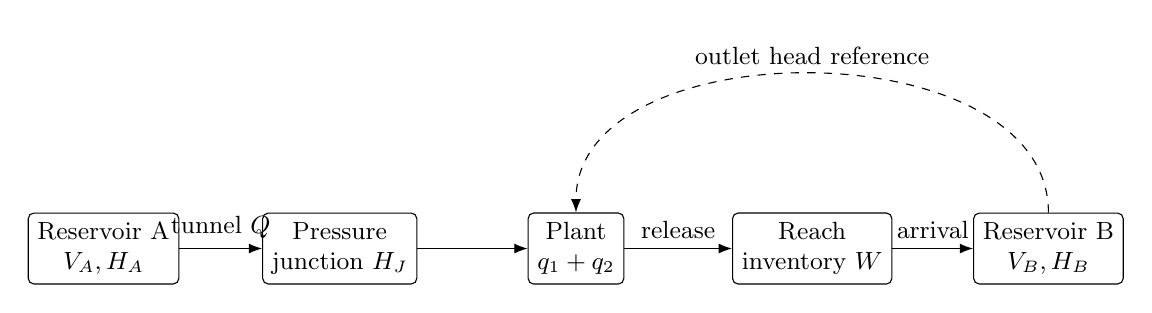
\begin{tikzpicture}[>=Latex,
 every node/.style={font=\small,align=center},
 box/.style={draw,rounded corners=2pt,minimum height=9mm}]
\node[box] (a) at (0,0) {Reservoir A\\$V_A,H_A$};
\node[box] (j) at (3,0) {Pressure\\junction $H_J$};
\node[box] (p) at (6,0) {Plant\\$q_1+q_2$};
\node[box] (r) at (9,0) {Reach\\inventory $W$};
\node[box] (b) at (12,0) {Reservoir B\\$V_B,H_B$};
\draw[->] (a) -- node[above]{tunnel $Q$} (j);
\draw[->] (j) -- (p);
\draw[->] (p) -- node[above]{release} (r);
\draw[->] (r) -- node[above]{arrival} (b);
\draw[->,dashed] (b.north) to[out=90,in=90]
 node[above]{outlet head reference} (p.north);
\end{tikzpicture}
\caption{Water destination and hydraulic reference have different roles.
Solid arrows move water; the dashed connection supplies the plant's outlet
head. Water reaches B after transport, although its level already affects
generation.}
\label{fig:network}
\end{figure}

\section{Pressure links and generating units}

\subsection{Tunnels and gates}

For an oriented tunnel $e=(v,w)$, positive $Q_e$ flows from $v$ to $w$.
At positive opening,
\begin{equation}
H_{vt}-H_{wt}=K_e(b_{et})Q_{et}|Q_{et}|,\qquad
K_e(b)=
\begin{cases}
R_e/b,&\text{without a gate-loss curve},\\
R_e+G_e(b),&\text{with a supplied gate-loss curve}.
\end{cases}
\label{eq:tunnel}
\end{equation}
$R_e>0$ and $G_e\ge0$ have units s$^2$/m$^5$.
The signed product ensures that friction opposes flow in either direction.
Continuity and these pressure equations determine flow sharing through
branches and loops; there is no independent allocation rule.

A closed gate instead imposes
\begin{equation}
b_{et}=0\ \Longrightarrow\ Q_{et}=0,\qquad
|Q_{et}|\le C_{et}.
\label{eq:closed}
\end{equation}
It imposes no equality of endpoint heads. A directed river outfall also has
$Q_{et}\ge0$. Tunnel positions are either prescribed or selected from a
finite declared set $\mathcal S_e\subset[0,1]$; arbitrary continuous tunnel
positions are not optimization decisions.

An instantaneous channel between reservoirs has a different supplied law:
\begin{equation}
X_{ct}=\Phi_c(H_{vt}-H_{wt},H_{{\rm ref},t}),\qquad
|X_{ct}|\le C_{ct}.
\label{eq:channel}
\end{equation}
The reference is explicitly either endpoint level. Each constituent
discharge curve is nondecreasing, passes through $(0,0)$ and preserves the
sign of the level difference. Responses may be asymmetric. Interpolation is
linear in level difference and between reference levels; endpoint segments
continue linearly in difference, while the nearest reference curve is held
outside the reference span. Channels have neither delay nor transit inventory.

\subsection{Energy conversion}

Let $q_{pt}=\sum_{g\in\mathcal G_p}q_{gt}$ and
$P_{pt}=\sum_{g\in\mathcal G_p}P_{gt}$. All units at plant $p$ share
\begin{equation}
h_{pt}=H_{{\rm source}(p),t}
       -\max\{H_{{\rm target}(p),t},h_p^{\rm floor}\}
       -T_p(q_{pt}).
\label{eq:nethead}
\end{equation}
Omit the floor when absent. $T_p\ge0$ is an additional tailwater rise, indexed
by total plant discharge; it is not the complete downstream elevation.
Shared penstocks are separate tunnels, whose loss therefore depends on the
combined flow through the penstock.

Unit operation is a disjunction,
\begin{align}
u_{gt}&\in\{0,1\},&
\underline q_{gt}u_{gt}&\le q_{gt}\le\overline q_{gt}u_{gt},&
\underline P_{gt}u_{gt}&\le P_{gt}\le\overline P_{gt}u_{gt}, \label{eq:onoff}\\
P_{gt}&=\gamma q_{gt}h_{pt}
          \eta_g(q_{gt},h_{pt})\,e_g(P_{gt}).&&&& \label{eq:power}
\end{align}
On, additionally enforce
\begin{equation}
\underline h_g\le h_{pt}\le\overline h_g,\qquad
\eta_g^{\min}\le\eta_g(q_{gt},h_{pt})\le1,\qquad
q_g^{\rm lo}(h_{pt})\le q_{gt}\le q_g^{\rm hi}(h_{pt})
\label{eq:unitdomain}
\end{equation}
The head and efficiency bounds always apply to running units; the flow
envelopes apply when supplied by a turbine table. Off, $q=P=0$ and these
operating inequalities are inactive; hydraulic heads remain in the network.

Turbine efficiency is either a table or the analytic relationship
\begin{equation}
\eta_g(q,h)=\eta_g^0
-\alpha_g\left(\frac{q-q_g^*}{q_g^*}\right)^2
-\beta_g\left(\frac{h-h_g^*}{h_g^*}\right)^2.
\label{eq:analyticeta}
\end{equation}
Tables are linear in head and linear or shape-preserving cubic in discharge.
Electrical efficiency $e_g$ is a separate piecewise-linear function of
\emph{electrical output}. Hence \eqref{eq:power} is implicit in $P$.
The accepted electrical curves make $P/e_g(P)$ strictly increasing,
so there is at most one admissible scalar conversion. If no curve is supplied,
$e_g=1$. This distinguishes turbine shaft conversion from electrical losses.

Plant state is the logical OR of its units:
\begin{equation}
U_{pt}\ge u_{gt}\ (g\in\mathcal G_p),\qquad
U_{pt}\le\sum_{g\in\mathcal G_p}u_{gt},\qquad U_{pt}\in\{0,1\}.
\label{eq:plantstate}
\end{equation}
Enforce $P_{pt}\le\overline P_{pt}$,
$q_{pt}\le\overline q_{pt}$ when supplied, and
$P_{pt}\ge\underline P_{pt}U_{pt}$,
$q_{pt}\ge\underline q_{pt}U_{pt}$.

\section{Reservoir outlets and river transport}

\subsection{Entry laws and confluences}

A reservoir-source reach has total entry
$R_{rt}=n_{rt}+d_{rt}$, where $n_{rt}$ is its natural inflow and
$d_{rt}$ is withdrawal from the reservoir. One chosen outlet law is
\begin{equation}
d_{rt}=
\begin{cases}
(C_{rt}-n_{rt})a_{rt},&\text{controlled outlet},\\
c_ra_{rt}\sqrt{\ell_{rt}},&\text{orifice},\\
c_r\ell_{rt}^{3/2},&\text{uncontrolled weir},\\
a_{rt}D_r(H_{{\rm source}(r),t}),&\text{supplied discharge curve}.
\end{cases}
\label{eq:outlets}
\end{equation}
Here $\ell=H_{\rm source}-z_r^{\rm crest}\ge0$, or
$\ell=\pos{H_{\rm source}-z_r^{\rm crest}}$ if dry operation is allowed.
An uncontrolled weir has $a=1$, including when a discharge table supplies its
law. Other openings satisfy their declared bounds in $[0,1]$.
Ordinary reaches obey $n_{rt}\le R_{rt}\le C_{rt}$.
Subtracting $d=R-n$, rather than $R$, in \eqref{eq:incidence} counts natural
river inflow exactly once.

For a confluence-fed reach, define local injection
\begin{equation}
L_{rt}=n_{rt}
       +\sum_{g\to r}q_{gt}+\sum_{e\to r}Q_{et},\qquad
R_{rt}=L_{rt}+\sum_{s\to r}\frac{A_{st}}{\kappa\Delta_t}.
\label{eq:confluence}
\end{equation}
Any number of upstream reaches and outfalls may merge. A confluence has one
outgoing reach; it does not decide how to split a stream. Delayed reaches
form a directed acyclic graph. Hydraulic loops through tunnels and
instantaneous channels remain admissible.

\subsection{Cohort response functions}

Travel time separates release from arrival. The response-function viewpoint
is classical~\cite{dooge}; here its precise discretization is part of the
model. Reference flows are nonnegative, strictly ordered and cover admissible
entry flows when more than one distribution is supplied. Delay edges are
nonnegative and strictly increasing. For reference flow $\rho_{rj}$, a supplied delay distribution is uniform
on each bin $[\delta_{rj\ell},\delta_{rj,\ell+1}]$ with probability
$w_{rj\ell}\ge0$, $\sum_\ell w_{rj\ell}=1$. Its cumulative distribution is
\begin{equation}
F_{rj}(s)=\sum_\ell w_{rj\ell}
\min\!\left\{1,\max\!\left\{0,
 \frac{s-\delta_{rj\ell}}{\delta_{rj,\ell+1}-\delta_{rj\ell}}\right\}\right\}.
\label{eq:cdf}
\end{equation}
With two or more reference flows, the mixture weights satisfy
\begin{equation}
\theta_{rkj}\ge0,\qquad \sum_j\theta_{rkj}=1,\qquad
R_{rk}=\sum_j\rho_{rj}\theta_{rkj},\qquad \theta_{rk}\in\SOS.
\label{eq:delayweights}
\end{equation}
Thus only neighboring distributions are blended. With a single distribution,
$\theta_{rk1}=1$ and there is no coordinate reproduction equation: its
reference flow does not fix the release. The selected mixture
stays with that cohort. Operating capacity changes do not rescale calibration
reference flows.

For a rectangular cohort released during $[\tau_k,\tau_{k+1})$, the fraction
arriving during interval $t$ at reference $j$ is
\begin{equation}
B_{rtkj}=\frac1{\Delta_k}\int_{\tau_k}^{\tau_{k+1}}
  \left[F_{rj}(\tau_{t+1}-s)-F_{rj}(\tau_t-s)\right]\dd s.
\label{eq:transfer}
\end{equation}
The arrival volume and instantaneous arrival rate are
\begin{align}
A_{rt}&=A^{\rm hist}_{rt}
+\kappa\sum_k\Delta_k R_{rk}\sum_j\theta_{rkj}B_{rtkj},
\label{eq:arrival}\\
f_r(s)&=f_r^{\rm hist}(s)+
\sum_k R_{rk}\sum_j\theta_{rkj}
 \left[F_{rj}(s-\tau_k)-F_{rj}(s-\tau_{k+1})\right].
\label{eq:pointarrival}
\end{align}
The integrals are evaluated exactly for the declared uniform bins.
Interpolating the \emph{fraction} and then multiplying by released flow makes
the transfer piecewise quadratic in $R$; interpolating already released
volumes would define a different response.

If every delayed reach has deterministic delay $\delta_r\ge0$, use event-shaped
entry streams $\widetilde R_r(s)$ and
\begin{equation}
f_r(s)=\widetilde R_r(s-\delta_r),\qquad
\widetilde R_r(s)=L_r(s)+\sum_{s'\to r}f_{s'}(s),\qquad
A_{rt}=\kappa\int_{\tau_t}^{\tau_{t+1}}f_r(s)\dd s
\label{eq:deterministic}
\end{equation}
at confluences for $s\ge0$. For $s<0$, $\widetilde R_r(s)$ is the
independently supplied entry history of that reach, not a backward evaluation
of the confluence recursion. On $[\tau_t,\tau_{t+1})$, a reservoir-source
stream is $\widetilde R_r(s)=n_{rt}+d_{rt}$, including natural inflow.
Link event streams to interval variables by
\begin{equation}
R_{rt}=\frac1{\Delta_t}\int_{\tau_t}^{\tau_{t+1}}\widetilde R_r(s)\dd s.
\label{eq:eventmean}
\end{equation}
Original pulses are shifted through successive confluences; they are not
replaced by interval averages. Zero and sub-interval delays therefore
produce genuine same-interval coupling. Entry-capacity restrictions are
also enforced on the event stream, including both sides of its jumps.

If any reach uses a distributed response, \eqref{eq:confluence} instead
mixes arrivals into new interval-average downstream cohorts.
Equations \eqref{eq:transfer}--\eqref{eq:arrival} remain exact for each such
cohort, but downstream timing is a grid approximation. Refining the mixing
grid and comparing cumulative arrivals and inventory estimates this error.
Mass conservation alone cannot detect an incorrectly spread pulse.

\subsection{Inventory, history and environmental flows}

Released water that has not arrived is still in the system:
\begin{equation}
W_{r,t+1}=W_{rt}+\kappa\Delta_t R_{rt}-A_{rt},\qquad
W_{r0}=W_r^{\rm hist}.
\label{eq:inventory}
\end{equation}
Historical entry cohorts supply initial inventory and future historical
arrivals: the historical terms in \eqref{eq:arrival} and
\eqref{eq:pointarrival} use the same formulas over supplied past intervals.
For a historical cohort $k$ on $[s_k,e_k)$, let $F_k$ be its selected delay
mixture. Then
\begin{equation}
W_r^{\rm hist}=\kappa\sum_{k\in\mathcal H_r}R_{rk}
\int_{s_k}^{e_k}\left[1-F_k(-s)\right]\dd s.
\label{eq:historyinventory}
\end{equation}
Unspecified earlier entry is zero in the declared model.
Each reach's history already includes its pre-horizon upstream
contributions; regenerating those contributions would double-count water.
Restart retains original executed cohorts and their release flows, as well
as reservoir states and operating histories. An average arrival bucket is
insufficient to reconstruct future arrival timing.

\paragraph{Conservation identity.}
Summing \eqref{eq:storage} and \eqref{eq:inventory} cancels every internal
transfer. Thus
\begin{equation}
\sum_i(V_{i,t+1}-V_{it})+\sum_r(W_{r,t+1}-W_{rt})
=\kappa\Delta_t\left(\sum_i I_{it}+\sum_r n_{rt}+E_t\right),
\label{eq:globalwater}
\end{equation}
where $E_t$ is net boundary exchange, positive into the modeled system.
For example, a plant outfall withdraws $q$ from its source, adds $q$ to reach
entry, and later leaves the reach as $A$; only that arrival enters the
receiving reservoir. Equation \eqref{eq:globalwater} follows by this same
cancellation for each arc, including reverse instantaneous flow.

Environmental restrictions may apply to reach entry $R_{rt}\ge R_{rt}^{\min}$,
window-average arrival, or instantaneous arrival:
\begin{equation}
\int_J f_r(s)\dd s\ge\int_J f_r^{\min}(s)\dd s,\qquad
f_r(s)\ge f_r^{\min}(s).
\label{eq:environment}
\end{equation}
Only the selected arrival policy applies. For prescribed rectangular cohorts,
distributed arrivals are piecewise linear; deterministic arrivals are
piecewise constant. Checking response and requirement breakpoints and the relevant one-sided
limits enforces the pointwise requirement for that transport model.
At the horizon endpoints use the interior limits.

A flow observation is an additional inequality, not a water injection:
\begin{equation}
\sum_{g\in\mathcal G_o}q_{gt}
+\sum_{r\in\mathcal D_o\cup\mathcal C_o}R_{rt}+I_{ot}
\ge M_{ot}.
\label{eq:observation}
\end{equation}
For an instantaneous channel, its observed release is $R_{ct}=X_{ct}$.
Named contributions must refer to water already represented in the network.

\section{Chronological operating constraints}

Define unit starts and stops relative to the supplied initial state:
\begin{equation}
u_{gt}-u_{g,t-1}=s^+_{gt}-s^-_{gt},\qquad
s^+_{gt}+s^-_{gt}\le1,\qquad s^\pm_{gt}\in\{0,1\}.
\label{eq:transitions}
\end{equation}
For every start at $\tau_t$, enforce $u_{gk}\ge s^+_{gt}$ whenever
$0\le\tau_k-\tau_t<L_g^{\rm up}$; for a stop, enforce
$u_{gk}\le1-s^-_{gt}$ whenever
$0\le\tau_k-\tau_t<L_g^{\rm down}$.
Initial state age fixes the remaining dwell interval.
Apply the same constraints to aggregate plant state $U$ when plant dwell
is declared. Changing the running member does not restart an already
operating plant. Dwell beyond the horizon is carried to a restart, rather
than forced by an invented terminal state.

Availability, forced states and prescribed output are hard restrictions:
\begin{equation}
\underline u_{gt}\le u_{gt}\le\overline u_{gt},\qquad
P_{gt}=P_{gt}^{\rm given},\quad q_{gt}=q_{gt}^{\rm given}
\label{eq:schedules}
\end{equation}
where supplied. Plant state also satisfies
$\underline U_{pt}\le U_{pt}\le\overline U_{pt}$;
plant output schedules constrain sums.
Maintenance forces the relevant units off. A zero schedule implies off;
a positive schedule implies on. All restrictions intersect, including
initial dwell; no input silently overrides another.

For interval-average discharge or release $x_t$, rate limits give
\begin{equation}
-\int_{m_{t-1}}^{m_t}r_x^-(s)\dd s
\le x_t-x_{t-1}\le
\int_{m_{t-1}}^{m_t}r_x^+(s)\dd s.
\label{eq:ramps}
\end{equation}
Unit and plant power use the same bounds with additional allowed jumps
$\sum_{g\in\mathcal G_x}\underline P_{gt}s^+_{gt}$ upward and
$\sum_{g\in\mathcal G_x}\underline P_{g,t-1}s^-_{gt}$ downward.
These allow the minimum running output at a transition, not unrestricted
startup or shutdown. Discharge and river ramps have no jump exemption.
The first comparison uses a supplied previous-window average and midpoint.
If absent, only that first comparison is omitted.

Reservoir volume ramps use $V_{i,t+1}-V_{it}$ and level ramps use
$Z_i(V_{i,t+1})-Z_i(V_{it})$, with rate integrals over
$[\tau_t,\tau_{t+1}]$. They constrain vertex changes, not continuous-time
derivatives.

For a tunnel interlock $\mathcal E_\ell$, with
$o_{et}=\mathbf1[b_{et}>0]$, require
\begin{equation}
\underline N_{\ell t}\le\sum_{e\in\mathcal E_\ell}o_{et}
\le\overline N_{\ell t}.
\label{eq:interlock}
\end{equation}
A positive position counts as open even when its flow is zero.

\section{Economic objective}

With price $\pi_t$ per MWh, reservoir and reach values $v_i,v_r$ per Mm$^3$,
and nonnegative movement and release-shortfall costs, maximize
\begin{align}
\mathcal V={}&\sum_t\pi_t\Delta_t\sum_g P_{gt}
-\sum_{g,t}\left(c^+_{gt}s^+_{gt}+c^-_{gt}s^-_{gt}\right)
-\sum_{e,t}c^b_{et}|b_{et}-b_{e,t-1}| \notag\\
&-\sum_{r,t}c^r_{rt}\xi_{rt}
+\sum_i v_i(V_{iT}-V_{i0})
+\sum_r v_r(W_{rT}-W_{r0}).
\label{eq:objective}
\end{align}
The first gate comparison uses its given initial position. Transition and
movement costs are charged once, without a duration multiplier.
A positive release penalty makes the entry minimum soft:
\begin{equation}
\xi_{rt}\ge0,\qquad
\xi_{rt}\ge\kappa\Delta_t(R_{rt}^{\min}-R_{rt}).
\label{eq:shortfall}
\end{equation}
$\xi$ is a volume in Mm$^3$; positive cost makes it the actual shortfall.
Without a positive penalty, the entry minimum remains hard and $\xi=0$.
Arrival minima and aggregate observations remain hard.

Terminal transit value prevents a release near the horizon from losing all
economic value merely because it has not yet arrived. These values are
explicit input assumptions. Subtracting initial inventories removes a
constant endowment from both reported value and its relative-gap denominator.

\section{Finite algebraic representation}
\label{sec:graphs}

The constraints above define a nonconvex MINLP. Discharge changes immediate
power, future head and sometimes travel response. Neither fixed commitment
nor exact interpolation makes these couplings convex.

\subsection{Exact interpolation graphs}

For a piecewise-linear curve with knots $(x_i,y_i)$, use
\begin{equation}
\lambda_i\ge0,\qquad \sum_i\lambda_i=1,\qquad
x=\sum_i x_i\lambda_i,\qquad y=\sum_i y_i\lambda_i,\qquad
\lambda\in\SOS .
\label{eq:sos}
\end{equation}
SOS2 means that at most two nonzero weights are allowed, and their indices
must be adjacent. It is a disjunctive interpolation constraint~\cite{huch}.
On one segment the coordinate equation determines those two weights, so
\eqref{eq:sos} gives the original curve value exactly.

Turbine tables use independent discharge weights $\lambda_i$ and head
weights $\mu_j$. Let $E_{ij}$ be knot efficiencies. A shape-preserving
cubic discharge interpolant~\cite{fritsch} has the representation
\begin{align}
w_i&=\lambda_i\lambda_{i+1},&
r_i&=\lambda_iw_i,\notag\\
\eta_j&=\sum_i E_{ij}\lambda_i+
\sum_i\left[A_{ij}r_i+B_{ij}(w_i-r_i)\right],&
\eta&=\sum_j\mu_j\eta_j .
\label{eq:cubic}
\end{align}
For segment width $\delta q_i=q_{i+1}-q_i$, secant
$d_{ij}=(E_{i+1,j}-E_{ij})/\delta q_i$ and original endpoint slopes
$m_{ij}$, the coefficients are
\begin{equation}
A_{ij}=\delta q_i(m_{ij}-d_{ij}),\qquad
B_{ij}=\delta q_i(d_{ij}-m_{i+1,j}).
\label{eq:hermitecoefficients}
\end{equation}
On an active pair, $\lambda_i+\lambda_{i+1}=1$, so the correction
basis is $\lambda_i^2\lambda_{i+1}$ and
$\lambda_i\lambda_{i+1}^2$, which spans the cubic corrections that vanish
at both endpoints. Off the active pair these products vanish.
For bilinear tables $A=B=0$. Clipping or extending a domain does not refit
the supplied slopes; outer discharge extensions use their declared secants.
Head extrapolation, where explicitly allowed, uses the outer head secant.
Off-state efficiency extensions are finite algebraic continuations, not
additional running-domain restrictions.

Compatible units share head coordinates, and each cohort shares one flow
coordinate across arrivals, pointwise requirements and terminal inventory.
The same construction represents piecewise-bilinear channel responses.
Auxiliary equalities in \eqref{eq:cubic}, the power equation and released
transport products remain nonlinear. SOS2 has not turned the problem into
a MILP. These graphs preserve the specified functions; valid inequalities
and branching improve the relaxation used to search them.

\subsection{Quadratic tunnel and gate graphs}

Signed losses can be expressed with a direction variable $z_{et}$:
\begin{equation}
Q=Q^+-Q^-,\quad
0\le Q^+\le Cz,\quad 0\le Q^-\le C(1-z),\quad
S=(Q^+)^2-(Q^-)^2,\quad z\in\{0,1\}.
\label{eq:signedloss}
\end{equation}
Then $S=Q|Q|$. Directed outfalls need only $S=Q^2$; known head ordering
can fix a direction. Finite gate selectors give both $b$ and its open
state $o$ as affine expressions. Define $d_o=o(H_v-H_w)$.
For bounds $L\le H_v-H_w\le U$, its exact binary-product hull is
\begin{equation}
Lo\le d_o\le Uo,\qquad
H_v-H_w-U(1-o)\le d_o\le H_v-H_w-L(1-o).
\label{eq:binaryhull}
\end{equation}
Together with $|Q|\le Co$ and $d_o=K(b)S$, this retains
\eqref{eq:tunnel}--\eqref{eq:closed}. $K(b)$ is affine in the
finite position selectors, with any finite coefficient assigned to the
closed position since $S=0$ there. Only quadratic product equalities are
needed. Wet/dry outlet branches similarly represent
$\ell=\max(H-z^{\rm crest},0)$; an auxiliary root $r\ge0$, $r^2=\ell$,
represents the square root in \eqref{eq:outlets}.

\subsection{Bounds that retain the physical equations}

Spatial branch-and-bound needs enclosing relaxations. Finite equipment and
storage domains, conservation and forward/backward inventory bounds supply
domains without restricting them to a previously found schedule.
Polynomial bounds include interior extrema, not only table knots.

Let $\overline e$ bound electrical efficiency and define the running-domain
power majorant $p^{\rm ub}(q,h)=\gamma\overline e\,qh\eta(q,h)$,
with nonnegative $q,h,\eta$. It is polynomial on each interpolation cell,
even when the electrical conversion is implicit.
If $p^{\rm ub}(q,h)\le aq+bh+c$, with $b\ge0$ and a full head lower bound $h_*$, then
\begin{equation}
P\le aq+b(h-h_*)+(c+bh_*)u
\label{eq:support}
\end{equation}
is valid for both states: on it bounds physical power; off $P=q=0$
and the right side is nonnegative. Bernstein polynomial enclosures can
bound the residual over each original interpolation cell to establish $c$.
A plane fitted only at samples does not establish this inequality.

A joint box envelope couples discharge, running head and efficiency.
Use exact binary-product hulls for $h_{\rm on}=uh$ and
$\eta_{\rm on}=u\eta$. Nonnegative corner weights $z_c$ satisfy
\begin{equation}
\begin{gathered}
\sum_c z_c=u,\quad \sum_c q_cz_c=q,\quad
\sum_c h_cz_c=h_{\rm on},\quad
\sum_c\eta_cz_c=\eta_{\rm on},\\
\gamma e_{\min}\sum_c q_ch_c\eta_cz_c
\le P\le\gamma e_{\max}\sum_c q_ch_c\eta_cz_c.
\end{gathered}
\label{eq:box}
\end{equation}
Up to eight corners describe a nonnegative running box, and
$e_{\min},e_{\max}$ bound electrical efficiency on its power interval.
A physical on point has product corner weights reproducing $qh\eta$;
off all weights vanish. The exact efficiency and power equalities remain.

Table-aware supports also share on-state head weights $\zeta_j$:
\begin{equation}
0\le\zeta_j\le\mu_j,\quad \sum_j\zeta_j=u,\quad
\sum_j(h_j-h_1)\zeta_j=h_{\rm on}-h_1u,\qquad
P\le aq+\sum_j c_j\zeta_j .
\label{eq:coordinatecuts}
\end{equation}
Coefficients enclose the complete polynomial power majorant, including corrections
between head nodes. On, $\zeta=\mu$; off, $\zeta=0$ while the hydraulic
head stays free. Analogous discharge-coordinate supports couple the same
power law along the other axis. A bounded separator may add further valid
supports. These constraints tighten relaxations; none replaces a physical
equality or adds a new operating decision.

\section{Solution, reconstruction and certificate}

JuMP supplies the algebraic Julia interface~\cite{jump}. SCIP solves the
global nonconvex model by branch-and-cut with spatial branching, nonlinear
relaxations and bound tightening~\cite{scip}. A preliminary MILP proposes
unit states and finite gate positions using approximate generation and
hydraulics. With those discrete decisions fixed, Ipopt solves nonlinear
dispatch~\cite{ipopt}. Several proposals can be dispatched under a shared
time allowance. Only proposals passing reconstruction and finer replay
are submitted as full-model starts.
The MILP objective is a surrogate, never an enclosing bound for
\eqref{eq:objective}. Fixed-discrete dispatch is a piecewise-smooth
nonconvex NLP, and a stationary point is not a global optimum.

Physical reconstruction then holds unit discharges and openings fixed and
advances the coupled equations chronologically. For each interval, a
Newton solve includes the next storage, pressure-junction heads, tunnel
flows and active outlet releases. Current arrivals remain in the solve
when travel time overlaps the same interval. Unobservable pressure
components receive one numerical reference while retaining every water
balance; admissible common pressure shifts respect junction bounds.
Electrical output is recovered from \eqref{eq:power}. Reusable numerical
arrays separate this equation evaluation from input parsing and solver
reporting.

Acceptance checks the original interval equations and operating restrictions,
then repeats integration on a finer grid with the original controls.
Schedules and ramps are compared over their original operating windows;
storage vertices, total water, cumulative arrivals and terminal transit
are checked separately. This prevents an apparently converged pressure
solve from concealing an operating violation or a transport error.
For prescribed tolerances $\varepsilon_V,\varepsilon_{\mathcal V}$, consistency
also requires
\begin{equation}
\begin{gathered}
\max_{i,t}|V_i^{\rm fine}(\tau_t)-V_{it}|\le\varepsilon_V,\qquad
\max_r|W_r^{\rm fine}(\tau_T)-W_{rT}|\le\varepsilon_V,\\
|\mathcal V^{\rm fine}-\mathcal V|
\le\varepsilon_{\mathcal V}\max(1,|\mathcal V|).
\end{gathered}
\label{eq:replaycriteria}
\end{equation}
Refinement supplies a numerical consistency test, not a rigorous enclosure
of continuous-time hydraulic error.

Let $L$ be the independently reconstructed value of a schedule feasible
for the declared interval model and $U$ a finite enclosing solver upper bound.
The reported gaps are
\begin{equation}
g_{\rm abs}=\max(0,U-L),\qquad
g_{\rm rel}=\frac{\max(0,U-L)}{\max(1,|L|)}.
\label{eq:gap}
\end{equation}
A numerical certificate requires an enclosing bound and the requested
absolute or relative gap. It concerns the declared interval model,
interpolation and finite gate sets. Fixing discrete decisions makes it
conditional on those decisions. The interval-model certificate and finer
replay acceptance are separate outcomes: a schedule with a certified objective gap can
still fail finer replay. Neither certifies a continuous-time optimum.
Floating-point solver tolerances and guarded polynomial bounds do not
constitute an interval-arithmetic proof.

\section{Discussion}

The useful separation is between the physical model, methods for finding
feasible controls, and methods for enclosing their optimum. Direct nonlinear
dispatch keeps head and efficiency changes inside the scheduling problem;
cohort accounting preserves water and its timing; exact interpolation graphs
retain the supplied response rather than silently fitting another one.
Independent reconstruction gives the delivered controls their physical
meaning, while global bounds quantify unresolved economic improvement.

These choices do not remove nonconvexity, make coarse river mixing exact,
or guarantee a short proof on a large network. Their benefit is a model whose
approximations and certificates can be stated together. Site calibration,
unmodeled hydraulic regimes and uncertainty remain separate questions.
The formulation can be extended by adding explicit physical laws and
operating constraints while retaining the same conservation, interpolation
and acceptance principles.

\begin{thebibliography}{9}
\bibitem{catalao}
J.~P.~S. Catal\~ao, H.~M.~I. Pousinho and V.~M.~F. Mendes.
Mixed-integer nonlinear approach for the optimal scheduling of a
head-dependent hydro chain.
\emph{Electric Power Systems Research} 80(8), 935--942, 2010.
\href{https://doi.org/10.1016/j.epsr.2009.12.015}{doi:10.1016/j.epsr.2009.12.015}.
\bibitem{dooge}
J.~C.~I. Dooge. A general theory of the unit hydrograph.
\emph{Journal of Geophysical Research} 64(2), 241--256, 1959.
\href{https://doi.org/10.1029/JZ064i002p00241}{doi:10.1029/JZ064i002p00241}.
\bibitem{fritsch}
F.~N. Fritsch and J. Butland.
A method for constructing local monotone piecewise cubic interpolants.
\emph{SIAM Journal on Scientific and Statistical Computing} 5(2), 300--304, 1984.
\href{https://doi.org/10.1137/0905021}{doi:10.1137/0905021}.
\bibitem{huch}
J. Huchette and J.~P. Vielma.
A combinatorial approach for small and strong formulations of disjunctive constraints.
\emph{Mathematics of Operations Research} 44(3), 793--820, 2019.
\href{https://doi.org/10.1287/moor.2018.0946}{doi:10.1287/moor.2018.0946}.
\bibitem{jump}
I. Dunning, J. Huchette and M. Lubin.
JuMP: A modeling language for mathematical optimization.
\emph{SIAM Review} 59(2), 295--320, 2017.
\href{https://doi.org/10.1137/15M1020575}{doi:10.1137/15M1020575}.
\bibitem{ipopt}
A. W\"achter and L.~T. Biegler.
On the implementation of an interior-point filter line-search algorithm
for large-scale nonlinear programming.
\emph{Mathematical Programming} 106, 25--57, 2006.
\href{https://doi.org/10.1007/s10107-004-0559-y}{doi:10.1007/s10107-004-0559-y}.
\bibitem{scip}
S. Vigerske and A. Gleixner.
SCIP: global optimization of mixed-integer nonlinear programs in a branch-and-cut framework.
\emph{Optimization Methods and Software} 33(3), 563--593, 2018.
\href{https://doi.org/10.1080/10556788.2017.1335312}{doi:10.1080/10556788.2017.1335312}.
\end{thebibliography}
\end{document}
